%%%%%%%%%%%%%%%%%%%
% K-WAY CLASSIFICATION
%%%%%%%%%%%%%%%%%%%
\def\title{Information [Relation] Extraction}
\begin{frame}{\title}
\hh{Input}:  Sentences containing (\subj{subject}, \obj{object}). \\
\hh{Output}: \rel{Relation} between \subj{subject} and \obj{object}. \\
\vspace{1em}
\pause

\begin{center}
  \w{\subj{I} 'm \obj{Australian}} $\implies$ \rel{per:origin}
\end{center}
\pause

\begin{center}
  \includegraphics[height=4cm]<1-2>{../img/hammer-placeholder.jpg}
  \includegraphics[height=4cm]<3-3>{../img/hammer.jpg}
  \includegraphics[height=4cm]<4-4>{../img/hammer-name.jpg}
\end{center}
\end{frame}


%%%%%%%%%%%%%%%%%%%
% OPEN IE
%%%%%%%%%%%%%%%%%%%
\def\title{Open Information Extraction}
\begin{frame}{\title}
\begin{center}
  \hh{More to life than a fixed relation schema} \\
  \vspace{0.5em}
  
\includegraphics[height=3cm]{../img/bartwindow.png} \\
\end{center}
\vspace{0.5em}
\pause

(\subj{Chris}, \rel{taught at}, \obj{Carnegie Mellon}) \\
(\subj{Chris}, \rel{taught at}, \obj{University of Sydney}) \\
(\subj{his research}, \rel{is on}, \obj{A broad range of statistical natural language topics})
\pause

(\subj{Obama}, \rel{was born in}, \obj{Hawaii}) \\
(\subj{young rabbits}, \rel{drink}, \obj{milk}) \\
(\subj{Heinz Fischer}, \rel{visits}, \obj{United States}) \\
\vspace{1em}
\end{frame}

%%%%%%%%%%%%%%%%%%%
% OPEN DOMAIN REL MOTIVATION
%%%%%%%%%%%%%%%%%%%
\def\title{What is OpenIE good for?}
\begin{frame}{\title}
\begin{center}
  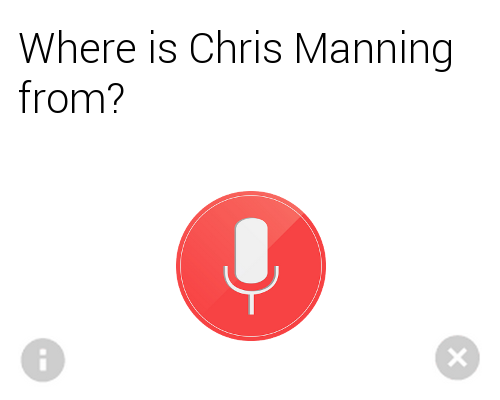
\includegraphics[width=7cm]{../img/google-chris-manning-origin.png}
\end{center}
\end{frame}
\begin{frame}{\title}
\begin{center}
  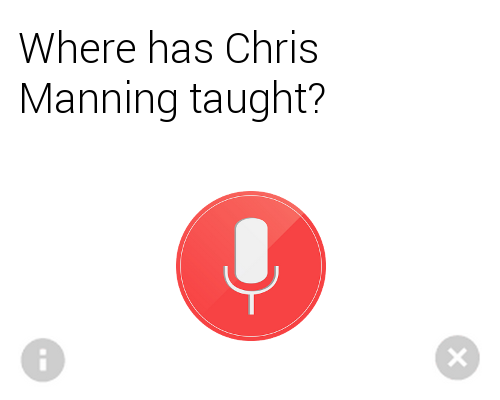
\includegraphics[width=7cm]{../img/google-chris-manning-taught.png}
\end{center}
\end{frame}
\begin{frame}[noframenumbering]{\title}
\begin{center}
  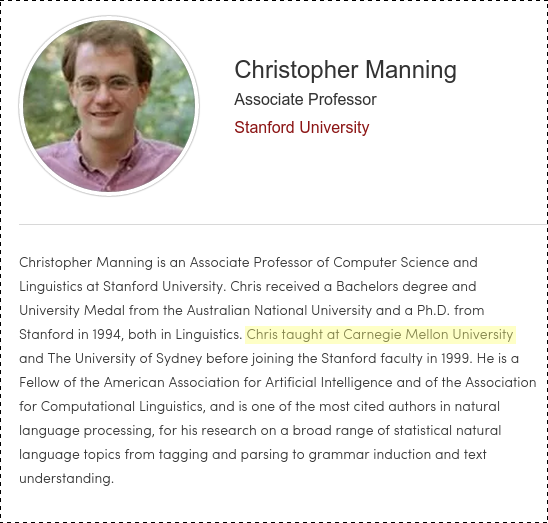
\includegraphics[height=7cm]{../img/chris-coursera-taught.png} \\
\end{center}
\end{frame}
\begin{frame}[noframenumbering]{\title}
\begin{center}
  
\includegraphics[width=7cm]{../img/google-chris-manning-research.png}
\end{center}
\end{frame}
\begin{frame}[noframenumbering]{\title}
\begin{center}
  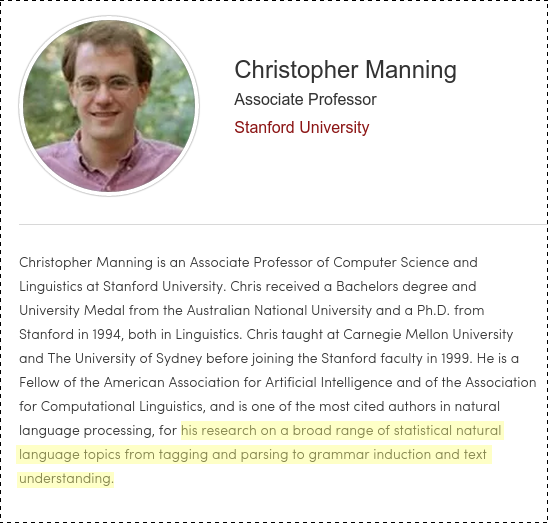
\includegraphics[height=7cm]{../img/chris-coursera-research.png} \\
\end{center}
\end{frame}

%%%%%%%%%%%%%%%%%%%
% PRIOR WORK
%%%%%%%%%%%%%%%%%%%
\def\title{Prior Work}
\begin{frame}{\title}

\hh{OpenIE (UW)}
\begin{itemize}
  \item TextRunner, ReVerb, Ollie, OpenIE 4.
  \item Learn surface and/or dependency patterns for triples.
\end{itemize}
\begin{center}
  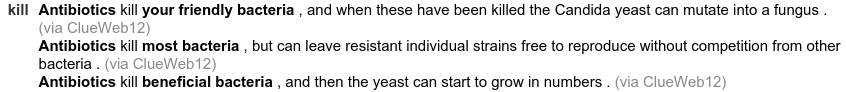
\includegraphics[width=8cm]{../img/openie-facts.png} \\
\end{center}
\pause

\hh{NELL (CMU)}
\begin{itemize}
  \item Bootstrapping an ontology from a small number of seed examples.
\end{itemize}
\begin{center}
  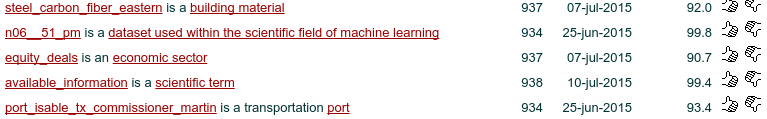
\includegraphics[width=8cm]{../img/nell-facts.png} \\
\end{center}

\end{frame}


%%%%%%%%%%%%%%%%%%%
% CHALLENGE: LONG SENTENCES
%%%%%%%%%%%%%%%%%%%
\def\title{Challenge: Long Sentences}
\begin{frame}{\title}
\hh{Short sentences are easy:}
\begin{center}
  \begin{dependency}[text only label,label style={above}]
    \begin{deptext}[column sep=-0.00cm]
      Obama \& was \& born \& in \& Hawaii \&[-1ex] . \\
    \end{deptext}
    \depedge[edge unit distance=2.25ex]{3}{5}{nmod:in}
    \depedge[edge unit distance=1.5ex]{3}{2}{cop}
    \depedge[edge unit distance=2.25ex]{3}{1}{nsubj}
    \depedge[edge unit distance=1.5ex]{5}{4}{case}
  \end{dependency}
\end{center}
\pause

\hh{But most sentences are longer:}
\begin{center}
  \begin{dependency}[text only label, label style={above}]
    \begin{deptext}[column sep=-0.00cm]
      Born \& in \& a \& small \& town \&[-1ex] , \& she \& took \& the \&
        midnight \& train \& going \& anywhere \&[-1ex] . \\
    \end{deptext}
    \depedge[edge unit distance=1.75ex]{1}{5}{nmod:in}
    \depedge[edge unit distance=1.5ex]{5}{4}{amod}
    \depedge[edge unit distance=2.25ex]{5}{3}{det}
    \depedge[edge unit distance=1.4ex]{8}{1}{vmod}
    \depedge[edge unit distance=2.5ex]{8}{7}{nsubj}
    \depedge[edge unit distance=2.25ex]{8}{11}{dobj}
    \depedge[edge unit distance=1.5ex]{11}{10}{nn}
    \depedge[edge unit distance=1.9ex]{11}{9}{det}
    \depedge[edge unit distance=1.5ex]{11}{12}{vmod}
    \depedge[edge unit distance=1.5ex]{12}{13}{dobj}
  \end{dependency}
\end{center}
\end{frame}


%%%%%%%%%%%%%%%%%%%
% CHALLENGE: LOST CONTEXT
%%%%%%%%%%%%%%%%%%%
\def\title{Challenge: Lost Context}
\def\deletable#1{\darkred{\hbox{\transparent{0.75} #1}}}
\begin{frame}{\title}
\hh{Sometimes annoying:}
\begin{center}
  \begin{dependency}[text only label,label style={above}]
    \begin{deptext}[column sep=-0.00cm]
      She \& was \& born \& in \& the \& small \& town \& 
      \deletable{of} \& \deletable{Springfield} \&[-1ex] . \\
    \end{deptext}
    \depedge[edge unit distance=2.25ex]{3}{1}{nmod:in}
    \depedge[edge unit distance=2.0ex]{3}{2}{cop}
    \depedge[edge unit distance=2.0ex]{3}{7}{nmod:in}
    \depedge[edge unit distance=2.25ex]{7}{6}{amod}
    \depedge[edge unit distance=2.5ex]{7}{5}{det}
    \depedge[edge unit distance=2.25ex,edge style={darkred!100!black,thick}]{7}{9}{nmod:of}
  \end{dependency}
\end{center}
\pause

\hh{Sometimes logically invalid:}
\begin{center}
  \begin{dependency}[text only label, label style={above}]
    \begin{deptext}[column sep=-0.00cm]
      All \& \deletable{young} \& rabbits \& drink \& milk \&[-1ex] . \\
    \end{deptext}
    \depedge[edge unit distance=1.75ex]{4}{3}{nsubj}
    \depedge[edge unit distance=1.75ex]{4}{5}{dobj}
    \depedge[edge unit distance=1.75ex,edge style={darkred!100!black,thick}]{3}{2}{amod}
    \depedge[edge unit distance=2.5ex]{3}{1}{det}
  \end{dependency}
\end{center}
\end{frame}

%%%%%%%%%%%%%%%%%%%
% CHALLENGE: TOO MUCH CONTEXT
%%%%%%%%%%%%%%%%%%%
\def\title{Challenge: Too Much Context}
\begin{frame}{\title}
\begin{center}
  \begin{dependency}[text only label, label style={above}]
    \begin{deptext}[column sep=-0.00cm]
      Heinz \& Fischer \& of \& Austria \& visits \& the \& United \& States \&[-1ex] . \\
    \end{deptext}
    \depedge[edge unit distance=2.00ex]{5}{2}{nsubj}
    \depedge[edge unit distance=2.25ex]{5}{8}{dobj}
    \depedge[edge unit distance=1.75ex]{2}{1}{nn}
    \depedge[edge unit distance=1.50ex]{2}{4}{nmod:of}
    \depedge[edge unit distance=1.75ex]{8}{7}{nn}
    \depedge[edge unit distance=2.00ex]{8}{6}{det}
  \end{dependency}

  (\subj{Heinz Fischer of Austria}; \rel{visits}; \obj{the United States})
\end{center}

\hh{Is this about Heinz Fischer or Austria?}
\pause
\begin{itemize}
  \item Is the subject a PERSON or LOCATION? \\
        (\subj{United States president Obama}; \rel{visits}; \obj{China})
  \pause
  \item Downstream applications don't want to deal with this.
  \item Downstream applications have less context to figure this out.
\end{itemize}
\end{frame}


%%%%%%%%%%%%%%%%%%%
% CHALLENGE: TOO MUCH CONTEXT
%%%%%%%%%%%%%%%%%%%
\def\title{Approach Open IE As \textit{Entailment}}
\begin{frame}{\title}
\hh{Challenge: Long Sentences}
\begin{itemize}
  \item Yield short, entailed clauses from sentences.
\end{itemize}
\vspace{0.5em}
\pause

\hh{Challenge: Lost Context}
\begin{itemize}
  \item Shorten these clauses only when logically valid.
\end{itemize}
\vspace{0.5em}
\pause

\hh{Challenge: Too Much Context}
\begin{itemize}
  \item Shorten these clauses as much as possible.
\end{itemize}
\vspace{0.5em}
\pause

\hh{\textit{No Longer A Challenge}}
\begin{itemize}
  \item Segment these short clauses into triples.
\end{itemize}
\end{frame}

%%%%%%%%%%%%%%%%%%%
% CLAUSE SPLITTING
%%%%%%%%%%%%%%%%%%%

\def\title{Yield clauses}
\begin{frame}{\title}
\begin{tabular}{ll}
\hh{Input:}  & Long sentence. \\
             & \w{Born in a small town, she took the midnight train going anywhere.} \\
\hh{Output:} & Short clauses. \\
             & \w{she Born in a small town.}
\end{tabular}

\begin{center}
  \only<1>{\treeBlank}
  \only<2>{\hspace{-1ex}\treeEdge}
  \only<3>{\hspace{-1.5ex}\treeSubj}
\end{center}
\end{frame}

%%%%%%%%%%%%%%%%%%%
% CLAUSE SEARCH
%%%%%%%%%%%%%%%%%%%
\def\title{Clause Classifier}
\begin{frame}{\title}
\begin{center}
  \only<1>{\begin{minipage}[t][3.5cm]{\textwidth}               \begin{center}\treeSubj     \end{center}\end{minipage}}
  \only<2>{\hspace{-1.0ex}\begin{minipage}[t][3.5cm]{\textwidth}\begin{center}\treeYield    \end{center}\end{minipage}}
  \only<3>{\hspace{-1.5ex}\begin{minipage}[t][3.5cm]{\textwidth}\begin{center}\treeYieldSubj\end{center}\end{minipage}}
  \only<4>{\hspace{-2.0ex}\begin{minipage}[t][3.5cm]{\textwidth}\begin{center}\treeYieldObj \end{center}\end{minipage}}
  \only<5>{\hspace{-2.5ex}\begin{minipage}[t][3.5cm]{\textwidth}\begin{center}\treeYieldRoot\end{center}\end{minipage}}
\end{center}

\vspace{-.5cm}
\begin{tabular}{ll}
\hh{Input:}  & Dependency arc. \\
\hh{Output:} & \textit{Action} to take.  \\
\end{tabular}
\pause

\begin{itemize}
  \item \textbf{Yield} (\w{you should brush your teeth}) \pause
  \item \textbf{Yield (Subject Controller)} (\w{Obama Born in Hawaii}) \pause
  \item \textbf{Yield (Object Controller)} (\w{Fred leave the room}) \pause
  \item \textbf{Yield (Parent Subject)} (\w{Obama is our 44th president})
\end{itemize}
\end{frame}


%%%%%%%%%%%%%%%%%%%
% MAXIMALLY SHORTEN CLAUSES
%%%%%%%%%%%%%%%%%%%
\def\title{Maximally Shorten Clauses}
\begin{frame}{\title}
\only<1>{\hh{\strut Some strange, nuanced function:}}
\only<2>{\hh{\strut An entailment function:}}
\only<3>{\hh{\strut A \darkblue{natural logic} entailment function:}} \\
\vspace{1em}

\begin{tabular}{lcl}
  \w{Heinz Fischer \textbf{of Austria}}      & $\implies$ & \w{Heinz Fischer} \\
  \w{\textbf{United States president} Obama} & $\implies$ & \w{Obama} \\
  \w{All \textbf{young} rabbits drink milk}  & \darkred{$\centernot \implies$} & \w{All rabbits drink milk} \\
  \w{Some \textbf{young} rabbits drink milk} & $\implies$ & \w{Some rabbits drink milk} \\
  \w{Enemies give \textbf{fake} praise}      & \darkred{$\centernot \implies$} & \w{Enemies give praise} \\
  \w{Friends give \textbf{true} praise}      & $\implies$ & \w{Friends give praise} \\
\end{tabular}
\end{frame}


%%%%%%%%%%%%%%%%%%%
% NATURAL LOGIC FOR DELETIONS
%%%%%%%%%%%%%%%%%%%
\def\title{Natural Logic For Clause Shortening}
\def\some{\monoUp{}{\textbf{Some$_{\uparrow \uparrow}$}}{}{}}
\def\rabbits{\monoUp{baby rabbits}{\footnotesize{young rabbits}}{rabbits}{mammals}}
\def\drink{\monoUp{slurp}{drink}{consume}{}}
\def\milk{\monoUp{Lucerne}{milk}{liquid}{something}}
\def\all{\monoUp{}{\textbf{All$_{\downarrow \uparrow}$}}{}{}}
\def\cats{\monoDown{house cats}{cats}{felines}{carnivores}}
\def\eat{\monoUp{slurp}{eat}{consume}{}}
\def\mice{\monoUp{fieldmice}{mice}{rodents}{placentals}}

\begin{frame}[noframenumbering]{\title}
\hh{Quantifiers determines the \textit{polarity} ($\uparrow$ or $\downarrow$) of words.} \\
\vspace{0.25cm}
\hh{Mutations must respect \textit{polarity}.} \\
\vspace{0.25cm}
\hh{Polarity determines valid deletions.}
\vspace{0.5cm}
\begin{center}
  \some \hspace{0.25cm} \rabbits \hspace{0.25cm} \drink \milk
\end{center}
\end{frame}

\def\rabbits{\monoUp{\footnotesize{young rabbits}}{\darkgreen{rabbits}}{mammals}{animals}}
\begin{frame}[noframenumbering]{\title}
\hh{Quantifiers determines the \textit{polarity} ($\uparrow$ or $\downarrow$) of words.} \\
\vspace{0.25cm}
\hh{Mutations must respect \textit{polarity}.} \\
\vspace{0.25cm}
\hh{Polarity determines valid deletions.}
\vspace{0.5cm}
\begin{center}
  \some \hspace{0.25cm} \rabbits \hspace{0.25cm} \drink \milk
\end{center}
\end{frame}

\def\rabbits{\monoDown{baby rabbits}{\footnotesize{young rabbits}}{rabbits}{mammals}}
\begin{frame}[noframenumbering]{\title}
\hh{Quantifiers determines the \textit{polarity} ($\uparrow$ or $\downarrow$) of words.} \\
\vspace{0.25cm}
\hh{Mutations must respect \textit{polarity}.} \\
\vspace{0.25cm}
\hh{Polarity determines valid deletions.}
\vspace{0.5cm}
\begin{center}
  \all \hspace{0.25cm} \rabbits \hspace{0.25cm} \drink \milk
\end{center}
\end{frame}

\def\rabbits{\monoDown{\footnotesize{young rabbits}}{\darkred{rabbits}}{mammals}{animals}}
\begin{frame}[noframenumbering]{\title}
\hh{Quantifiers determines the \textit{polarity} ($\uparrow$ or $\downarrow$) of words.} \\
\vspace{0.25cm}
\hh{Mutations must respect \textit{polarity}.} \\
\vspace{0.25cm}
\hh{Polarity determines valid deletions.}
\vspace{0.5cm}
\begin{center}
  \all \hspace{0.25cm} \rabbits \hspace{0.25cm} \drink \milk
\end{center}
\end{frame}

%%%%%%%%%%%%%%%%%%%
% CHALLENGE: SOLVED
%%%%%%%%%%%%%%%%%%%
\def\title{Approach Open IE As \textit{Entailment}}
\begin{frame}{\title}
\hh{Challenge: Long Sentences}
\begin{itemize}
  \item[\checkmark] Yield short, entailed clauses from sentences.
\end{itemize}
\vspace{0.5em}

\hh{Challenge: Lost Context}
\begin{itemize}
  \item[\checkmark] Shorten these clauses only when logically valid.
\end{itemize}
\vspace{0.5em}

\hh{Challenge: Too Much Context}
\begin{itemize}
  \item[\checkmark] Shorten these clauses as much as possible.
\end{itemize}
\vspace{0.5em}

\hh{No Longer A Challenge}
\begin{itemize}
  \item Segment these short clauses into triples.
\end{itemize}
\end{frame}

%%%%%%%%%%%%%%%%%%%
% CHALLENGE: SOLVED
%%%%%%%%%%%%%%%%%%%
\def\title{No Longer A Challenge}
\begin{frame}{\title}
\begin{center}
\begin{tabular}{lcl}
  \w{Heinz Fischer visited US} & $\implies$ & 
    (\subj{Heinz Fischer}; \rel{visited}; \obj{US}) \\\pause
  \w{Obama born in Hawaii} & $\implies$ & 
    (\subj{Obama}; \rel{born in}; \obj{Hawaii}) \\\pause
  \w{Cats are cute} & $\implies$ & 
    (\subj{Cats}; \rel{are}; \obj{cute}) \\\pause
  \w{Cats are sitting next to dogs} & $\implies$ & 
    (\subj{Cats}; \rel{are sitting next to}; \obj{dogs}) \\\pause
    & $\dots$ & 
\end{tabular}
\vspace{2em}

\hh{6 dependency patterns (+ 8 nominal patterns)}
\end{center}
\end{frame}

%%%%%%%%%%%%%%%%%%%
% DO WE NEED TRIPLES
%%%%%%%%%%%%%%%%%%%
\def\title{Useful Without Triples}
\begin{frame}{\title}
\hh{Simple, short sentences are themselves useful}
\begin{itemize}
\item $\dots$ for relation extraction (Miwa et al. 2010).
\item $\dots$ for textual entailment (Hickl and Bensley, 2007).
\item $\dots$ for summarization (Siddharthan et al. 2004).
\end{itemize}
\vspace{0.5cm}
\pause

\hh{Two use-cases:}
\begin{center}
\begin{tabular}{cc}
\textbf{Triples for Logical Reasoning} & \textbf{Text for Surface Reasoning} \\
& \\

\includegraphics[width=2cm]{../img/database.png} & 
  
\includegraphics[width=2cm]{../img/books.png}
\end{tabular}
\end{center}

\end{frame}


%%%%%%%%%%%%%%%%%%%
% EVALUATION INTRO
%%%%%%%%%%%%%%%%%%%
\begin{frame}{Problem}
\begin{center}
How do you evaluate open domain triples?
\end{center}
\end{frame}

\def\title{Extrinsic Evaluation: Knowledge Base Population}
\begin{frame}[noframenumbering]{\title}
\begin{center}
\begin{tabular}{cccc}
  \begin{tabular}{c}
    \h{Unstructured Text} \\
    \\
    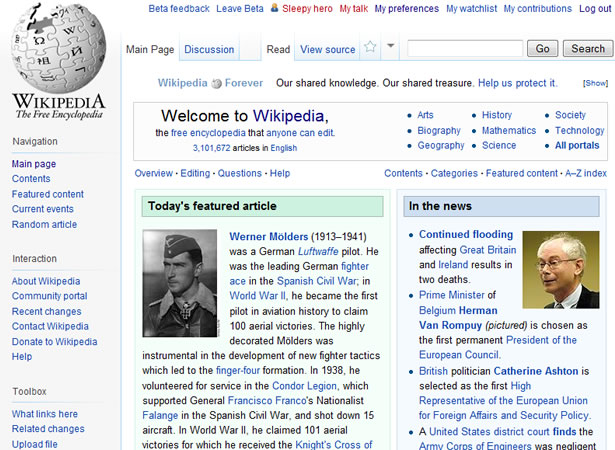
\includegraphics[width=2cm]{../img/wiki.jpg} \\
    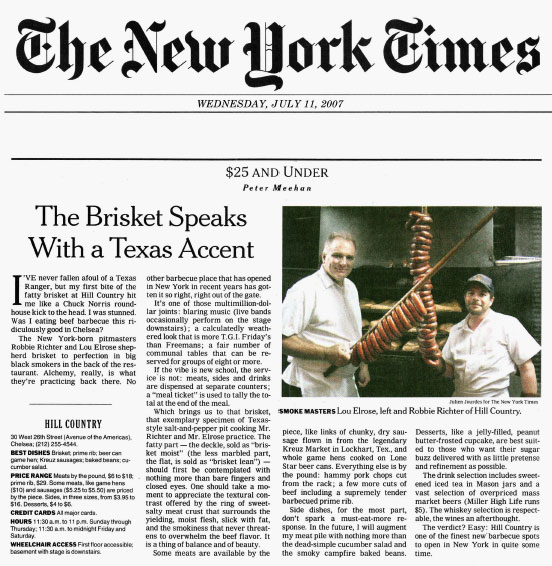
\includegraphics[width=2cm]{../img/nyt.jpg} \\
    
\includegraphics[width=2cm]{../img/blog.jpg}
  \end{tabular} &

  \Huge{$\Rightarrow$} &
  
  \begin{tabular}{c}
  \h{Structured Knowledge Base} \\
  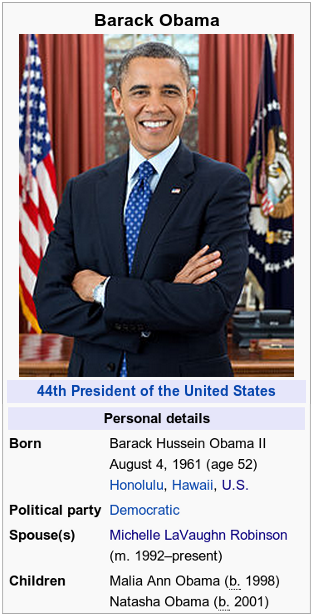
\includegraphics[width=2.75cm]{../img/obama-infobox.png}
  \end{tabular}
\end{tabular}
\end{center}
\end{frame}

\begin{frame}[noframenumbering]{\title}
\hh{Relation Extraction Task:}
\begin{itemize}
  \item Fixed schema of 41 relations.
  \item Precision: answers marked correct by humans.
  \item Recall: answers returned by any team (including LDC annotators).
\end{itemize}
\pause
\vspace{1em}

\hh{Comparison:} \textit{Open Information Extraction to KBP Relations in 3 Hours}.
  (Soderland et. al)

\begin{center}
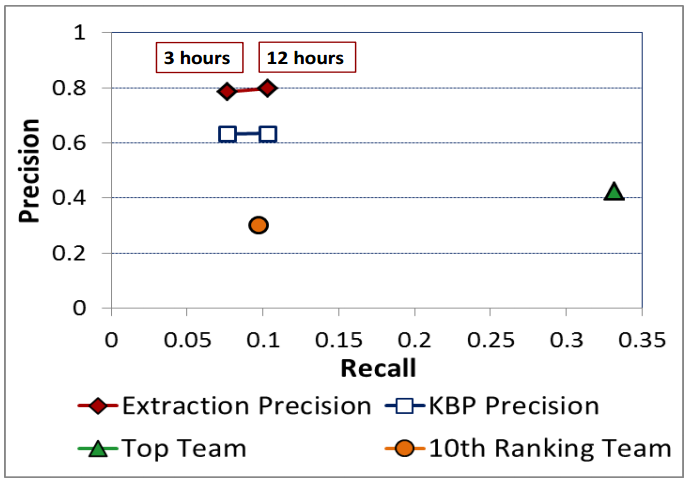
\includegraphics[scale=0.20]{../img/uw-openie.png} \\
\end{center}
\end{frame}

%%%%%%%%%%%%%%%%%%%
% RELATION MAPPING
%%%%%%%%%%%%%%%%%%%
\def\title{Prerequisite Task: Open IE $\rightarrow$ KBP Relations}
\begin{frame}{\title}
\begin{enumerate}
  \item Hand-coded mapping. \\
        (Same as UW; both over 1-2 weeks)
        \pause
        \vspace{1em}

  \item Learned relation mapping.
  \begin{itemize}
    \item For each type signature $t_1, t_2$;
    \item For an open IE relation $r_o$ and KBP relation $r_k$;
    \pause
    \item Compute:
      \begin{center}
        $
        p(r_k, r_o \mid t_1, t_2) = \frac{
          \textrm{count}(r_k, r_o,  t_1, t_2)
        }{
          \sum_{r_k', r_o'}\textrm{count}(r_k', r_o', t_1, t_2)
        }
        $.
      \end{center}
    \pause
    \item Rank by PMI$^2(r_o, r_k \mid t_1, t_2)$:
      \begin{center}
        $
        \textrm{PMI}^2(r_k, r_o \mid t_1, t_2) = \log \left( \frac{p(r_k, r_o \mid t_1, t_2)^2}{p(r_k \mid t_1, t_2) \cdot p(r_o \mid t_1, t_2)} \right)
        $.
      \end{center}
  \end{itemize}
\end{enumerate}
\end{frame}

\begin{frame}[noframenumbering]{\title}
\begin{center}
\begin{tabular}{l:lc}
  \textbf{KBP Relation} & \textbf{Open IE Relation} & \textbf{PMI$^2$}\\
  \hline
  \small{\rel{Per:Date\_Of\_Birth}}    & \ww{be bear on} & 1.83       \\
                                       & \ww{bear on} & 1.28          \\
  \small{\rel{Per:Date\_Of\_Death}}   & \ww{die on} & 0.70  \\
                                      & \ww{be assassinate on} & 0.65  \\
  \small{\rel{Per:LOC\_Of\_Birth}}     & \ww{be bear in} & 1.21        \\
  \small{\rel{Per:LOC\_Of\_Death}}     & \ww{\darkred{*elect president of}} & 2.89                \\
  \small{\rel{Per:Religion}}          & \ww{speak about} & 0.67   \\
                                      & \ww{popular for} & 0.60   \\
  \small{\rel{Per:Parents}}            & \ww{daughter of}     & 0.54          \\
                                      & \ww{son of} & 1.52          \\
  \small{\rel{Per:LOC\_Residence}}     & \ww{of} & 1.48       \\
                                       & \ww{\darkred{*independent from}} & 1.18    \\
\end{tabular}
\end{center}
\end{frame}

%%%%%%%%%%%%%%%%%%%
% RESULTS
%%%%%%%%%%%%%%%%%%%
\def\title{Results}
\begin{frame}{\title}
\hh{TAC-KBP 2013 Slot Filling Challenge:}
\begin{itemize}
  \item End-to-end task -- includes IR + consistency.
\item \textbf{Precision:} facts LDC evaluators judged as correct. \\
      \textbf{Recall:} facts other teams (including LDC annotators) also found.
\end{itemize}
\vspace{0.25cm}

\def\bell{\raisebox{-2.5mm}{
\includegraphics[height=5mm]{../img/bell.png}}}
\def\whistle{\raisebox{-2.5mm}{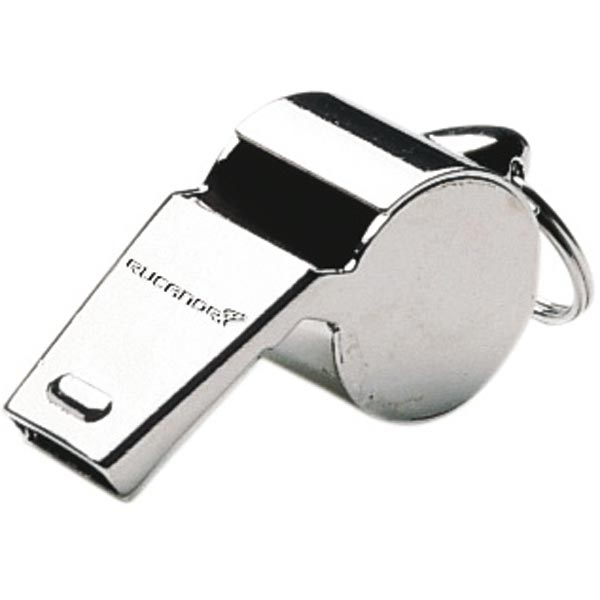
\includegraphics[height=5mm]{../img/whistle.jpg}}}
\begin{center}
\begin{tabular}{lrrr}
\hline
\textbf{System}                & \multicolumn{1}{c}{\textbf{P}}    
                               & \multicolumn{1}{c}{\textbf{R}}    
                               & \multicolumn{1}{c}{\textbf{F$_1$}} \\
\hline
UW Submission                   & 69.8          & 11.4          & 19.6 \\
Ollie                           & 57.7          & 11.8          & 19.6 \\
\pause
\darkblue{Our System}           & \darkblue{61.9} & \darkblue{13.9} & \darkblue{22.7} \\
\hline
\pause
Median Team                     &               &               & 18.6 \\
\darkblue{Our System} + \bell\ + \whistle  & \darkblue{58.6} & \darkblue{18.6} & \darkblue{28.3} \\
Top Team                        & 45.7          & 35.8          & 40.2 \\
\hline
\end{tabular}
\end{center}
\end{frame}
